\section{Labour market characteristics} \label{isect3}

In addition to the political and social upheavals caused by the civil war and mass migration, the time period 1998-2018 encapsulates a major shift of economic activity, from a low-productivity agriculture sector to a high-productivity service sector. In that time, the agriculture sector declined by 8 percentage points from 34\% in 1998, whereas the service sector increased from 8\% to 13\% for market services \footnote{Market service includes trading considering both retail and wholesale services, transportation, financial sector including banking, financing and insurance, repair and maintenance, communication including broadcasting, information technology, and repairs and maintenance.} and 25\% to 37\% for non-market services \footnote{Non-market services consists of public administration, defence, education, health and social services. Both government and private sector provide education and health service in Nepal. This definition nods to the fact that government covers larger share.}. This trend of transformation was not geographically uniform. In 1998, women in rural areas were predominantly in agriculture, whereas women in urban areas were mostly in the health, education, government, and manufacturing sectors. As time passed, however, the importance of manufacturing declined substantially in both urban and rural areas. The manufacturing jobs in urban areas were mostly in the textile and garment industry, which collapsed after the end of the Multifiber Arrangement in the early 2000s~\citep{shakya2018death}. Industry-wise, women in 2018 were employed in health, education, and government jobs in both areas; see figure \ref{fig:industryUrbRur}; since 2008 and the introduction of the reservation system, these sectors have absorbed women on a large scale~\citep{Subedi2022}. Another important employer of women are banking and private enterprises, primarily in urban areas.\par   
	
The economic transformation also changed the nature of available work. In 1998, approximately 50\% of the jobs were elementary occupations, usually in agriculture, while managers, professionals, and technicians only accounted for 21\% of the jobs. In the subsequent two decades, non-skilled employment decreased by 5\% and managerial jobs increased by almost 12\%. In 1998, women were primarily engaged in non-skilled work (see figure \ref{fig:occupationUrbRur}); by 2018, jobs that employed women in rural areas were divided into elementary occupations and the newly-growing white-collar jobs.\par 

\begin{figure}[htb!]
	\centering
	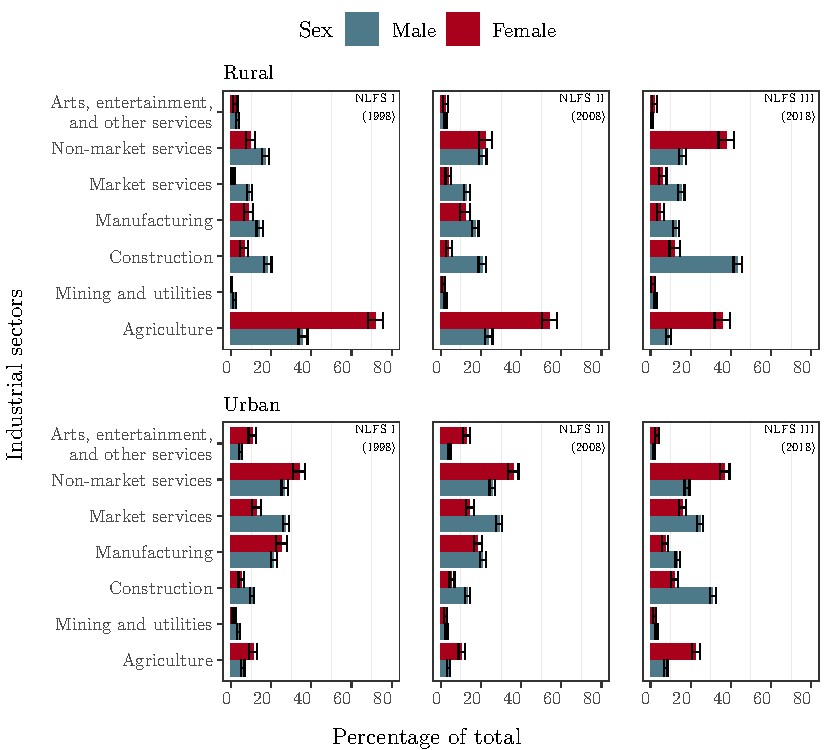
\includegraphics{./figure/industryUrbRur_bar_all_all}
	\caption{Industry-wise employment in rural and urban areas}
	\label{fig:industryUrbRur}
\end{figure}


\begin{figure}[htb!]
	\centering
	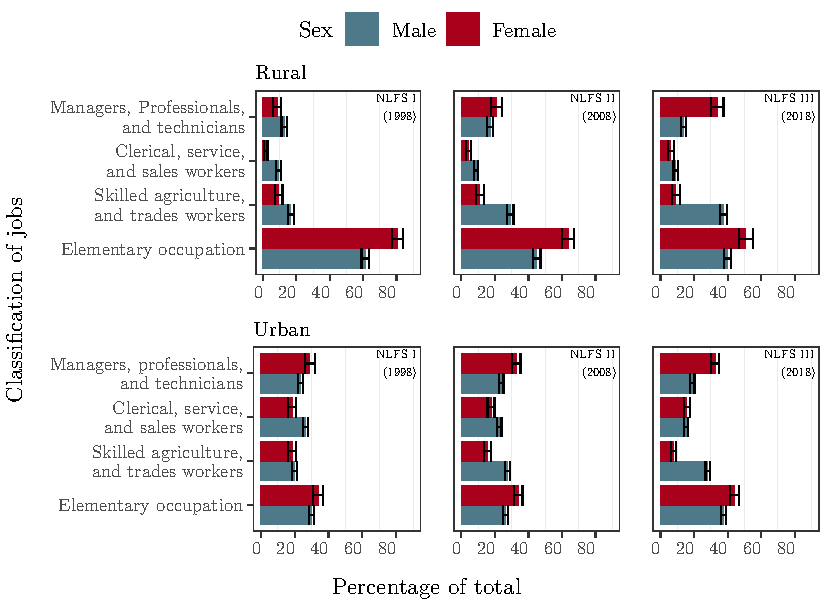
\includegraphics{./figure/occupationUrbRur_bar_all_all}
	\caption{Classification of jobs in rural and urban areas}
	\label{fig:occupationUrbRur}
\end{figure}

After the restoration of democracy in 1990, the country went through a liberalisation and decentralisation of its education sector, with a marked shift in attitude toward education: it was no longer just a social service, but an investment with its own economic returns. This change fostered the growth of the private education sector, particularly in urban areas, catering to families in the burgeoning middle and higher classes~\citep{Carney2009}. The decentralization policies were also well-received -- especially by rural communities, since the policies involved greater community participation in building and operating education institutions, enrolling first-generation graduates all over Nepal. Moreover, during this time, newly available jobs in the service sector that paid more for extra years of schooling created a strong case for higher education, especially among women. Thus, the gender gap in education has progressively narrowed over time (see figure A2 in annex), with both men and women attaining higher levels of education. However, as time has gone on, employed women have outpaced employed men in higher education. This educational phenomenon is not surprising: community colleges have class cohorts with more than two-thirds women, other degree-granting institutions having gender parity~\citep{Ugc2022}.\par 

%\input{tables/laborForceParticipation.tex} 
	
The increase in the number of years of schooling also led the young working-age cohort to stay in education for longer, delaying their entry into the job market. This delay, together with the transition of the economy away from the low-yielding agriculture sector, caused a gradual decline in the labour force participation rate from 50.2\% to 32.4\% over the two decades. By 2018, women’s labour force participation was at 18.2\% from the earlier 31.3\%, whereas men saw even larger decline (from 70.4\% to 50.9\%). Of those who are in the labour force, a complete reversal has occurred in its composition: in 1998, the majority of men and more than two-thirds of women in the labour force were self-employed; by 2018, a majority of men and a larger number of women reported being engaged in wage jobs than self-employment (see table A1 in annex). Overall, between 1998 and 2018, fewer people participated in the labour force, but among those who do, more are in wage-paying jobs than self-employment.\par    

\begin{figure}[htb] 
	\centering
	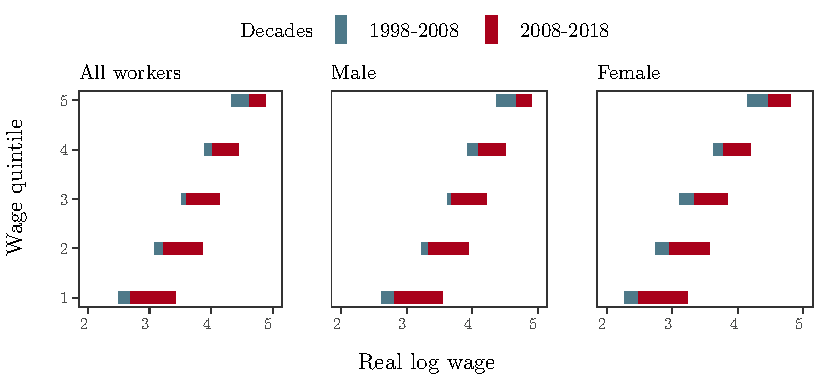
\includegraphics{./figure/log_real_wage_change_NLFS_all}
	\caption{Changes in real wage throughout the wage distribution (1998-2018)}
	\label{fig:wagechangeAll}
\end{figure} 

In the two decades we investigated, wage-earners saw their earnings improve in real terms. The increase in wages in the first decade was negligible: only the highest quintile saw sustained progress which exacerbated the inter-quintile wage spread, especially among men (see table A2 in annex). In terms of gender, women more greatly benefited from the changes in the first decade (see figure \ref{fig:wagechangeAll}). In contrast, between 2008 and 2018, we see substantial wage improvements for both genders across all quintiles. In this decade too, women saw larger gains, and they improved their position relative to men. Women in the highest wage quintile experienced substantial wage improvements and came quite close to the highest-earning men. Consequently, the gender wage gap decreased all around, with the sharpest decline in the highest quintile group. With time, the wage distributions shifted, and the largest improvement came at the lower end of the distribution. This pro-poor shift compressed real wages across both genders, negating the increase in the wage spread of the first decade.\par

Wage evolutions differed substantially between rural and urban areas (see figure A1 in the annex). In the first decade, development in urban areas was anti-poor, with people in the bottom three quintiles seeing either stagnant or eroding real wages. At the same time, rural areas saw improvements across all groups that brought them closer to the urban wages. In the second decade, wages improved across both areas, but larger rural gains narrowed the urban-rural wage divide. A probable cause for this narrowing is the out-migration (mostly of men) that largely occurred in the second decade. This out-migration decreased the rural labour supply, pushing rural wages up toward parity with urban wages. See table \ref{tab:SummarySSVE} for further details on observed characteristics across years.\par 

%On an average, employed males are generally 3 years older than employed females, which is consistent in each survey rounds; see table \ref{tab:SummarySSVE}. But, the average age of employed has increased approximately by 2 years for both genders in the same time. Also, the employed females in 2018, who are overwhelmingly from urban areas, come from families with household heads who are more educated than their male counterparts. In terms of ethnicity, there has been increased employment among Madheshi and Dalit individuals between 1998 and 2008, with further improvement specifically for the Dalit community in 2018. Generally, Khas and Janajati males dominate the job market.\par





